This section is devoted to review the particularities of the Simulated Binary Crossover (SBX) discussed in this work.
%
Thereafter, are briefly explained some popular algorithms, one of them widely used in mono-objective problems, and the rest designed for multi-objective problems.

\subsection{Multi-objective Evolutionary Algorithms}
Currently, there exist a large number of MOEAs that follows different design principles.
%
In orde to better classfy them, several taxonomies have been propose ref21.
%
Attending to the principles of design, MOEAs can be based on Pareto dominance, indicators and/or decomoposition ref4.
%
Currently, none of these methods have reported a clear advantage over the other ones.
%
Particuarly, the experimental validation has been carry out by including the Non-Dominated Sorting Genetic Algorithm (NSGA-II) ref, the MOEA based on Decomposition ref, and the $S$-Metric Selection Evolutionary Multi-objective Optimization Algorithm (SMS-EMOA) ref.
%
Therefore, they are repsentative methos of the domination-based, decomposition-based and indicator based paradigms, respectively.

\subsection{Domination-Based MOEAs - NSGAII}

One of the most reconized paradigms are the domination based algorithms, particularly this family are based on the application of the dominance relation to design different components of the EAs.
%
Since the dominance relation does not inheritly promotes diversidy in the objective space, auxiliary techniques such as niching crowding and/or clustering are usually integrated with the aim of obtain an aceptable spread and diversity in the solution space.
%
One of the most problematic issues of implement the dominance relation is related with the number of objectives, therefore if the number of function objective increase the selection pressure is decremented considerabily, based in this some strategies have been developed to deal with the many-objective problems.

%
Probably, the most popular technique of this group is the NSGA-II.
%
This algorithm ref2 implement a special parent selection operator.
%
This operator is based on two mechanism: fast-non-dominated-sort and crowding.
%
The first one tend to provide a convergence and the second one promotes the presetvation of diversity in the objective space.
%
Last versions is the NSGA-II and is designed to deal with many-objective problems.
%

\subsection{Decomposition-Based MOEAs - MOEA/D}

Decomposition-based MOEAs ref transform a MOP in a set of single-objective optimization problems that are considered simultaneously ref3.
%
This tranformation can be achieved throguh several approaches.
%
The most popular of them is based in a weighted Tchebycheff function, therefore it is necessary provide weigth vectors well distribuited with the aim of obtain well-spread solutions.
%
However, this is a difficulty of these kinds of approaches because the quality of the aproximation is related with the weight vectors.
%
MOEA/D ref25 is a recently designed decomposition-base MOEA.
%
Its main principles include problem decomposition, weighted aggregation of objectives and mating restrictions throguh the use of neighborhoods.
%
Particularly, the neighborhoods are considered in the variation operators.
%
A very used variant of the MOEA/D is the MOEA/D-DE, which use the DE operators (lampinen ref) and polynomial mutation operator for producing new solutions, also it has two extra measures for maintaining the population diversity (refs polynomial mutation).
%
However these two extra mechanism are not enough to deal with long-term executions.


\subsection{Indicator-Based MOEAs - SMS-EMOA}

In multi-objective optimization several quality indicators have been developed to compare the performance of MOEAs.
%
Since these indicators measure the quality of the approximations attained by MOEAs, a paradigm based on the application of these indicators was proposed.
%
Particularly, instead of dominance concept, the indicators are used in the MOEAs to guide the optimization process.
%
Among the different indicators, hypervolume is a widely accepted Pareto-compliance quality indicator.
%
The principal advantage of this algorithms is that the indicator usually takes into account both the quality and diversity of the solutions.
%

A popular and extensively used indicator-based algorithm is the SMS-EMOA ref.
%
This algorithm might be considered as hybrid, since it involves an indicator and dominance concepts.
%
Scencially it integrates the non-dominated sorting with the use of the hypervolume metric.
%
Thus, SMS-EMOA uses the hypervolume as a density estimator which results in a computationally extensive task.
%
Taking into account the promising behavior of SMS-EMOA, it has been used in our experimental validation.
%


\subsection{Analysis of the Simulated Binary Crossover SBX}

The principal components involved in the search process of a GA are the reproduction operators.
%
Specifically, the crossover and mutation operators are highly related with quality and diversity issues ref.
%
Particularly, in this paper is addresed the crossover operator.

The Simulated Binary Crossover (SBX) ref is popularly implemented in GAs ref.
%
The SBX is classified as Parent-Centric, meaning that two offspring values ($c_1$ and $c_2$) are created around the parent values ($p_1$ and $p_2$).
%
Also the process of generate the offspring values is based in a probability distribution.
%
This distribution is defined by a non-dimensional variable, better known as the spread factor $\beta = |c_1 - c_2 | / |p_1 - p_2|$, indicating the ratio of the spread children values to the parent values.
%

Additionally, this density function uses a distribution index $\eta$ (user-defined control parameter) that alters the exploration capability of the operator.
%
Specifically, a small index induce a larger probability of building offsprings values more dissimilar than parents values, whereas with a high index the probabilities of generating offspring solutions that are similar to the parents increse.
%

Principally, the SBX has non-zero probability of creating any number in the search space by recombining any two parent values from the search space.
%
The probability distribution to create an offspring value is defined as a function of a non-dimensionalized parameter $\beta \in [0, \infty]$ as follows:
%
\begin{equation}
    P(\beta)= 
\begin{cases}
     0.5(\eta_c + 1)\beta^{\eta_c},& \text{if} \quad \beta \leq 1\\
     0.5(\eta_c + 1) \frac{1}{\beta^{\eta_c + 2}} ,& \text{otherwise}
\end{cases}
\end{equation}
%
Based in the mean-preserving property of offspring values and parent values, the distribution probability preserve the following properties:
\begin{itemize}
\item Both offspring values are equi-distant from parent values.
\item There exist a non-zero probability to create offspring solutions in the entire space  from any two parent values.
\item The overall probability of creating a pair offspring values within the range of parent values is identical to the overall probability of creating two offspring values outside  the range of parent values.
\end{itemize}

Therefore, considering two participating parent values ($p_1$ and $p_2$), two offspring values ($c_1$ and $c_2$) can be created as linear combination of parent values with a random number $u \in [0, 1]$, as follows:
\begin{equation} 
\begin{split}
c_1 &= 0.5(1 + \beta(u))p_1 + 0.5(1 - \beta(u)) p_2 \\
c_2 &= 0.5(1 - \beta(u))p_1 + 0.5(1 + \beta(u)) p_2
\end{split}
\end{equation}

The parameter $\beta(u)$ depends on the random number $u$, as follows:
\begin{equation}
    \beta(u)= 
\begin{cases}
     (2u)^{\frac{1}{\eta_c+1}},& \text{if} \quad u \leq 0.5,\\
     	(\frac{1}{2(1-u)})^{\frac{1}{\eta+1}} ,& \text{otherwise}
\end{cases}
\end{equation}

The above equation only considers a optimization problem having no variable bounds.
%
In most practical problems, each variable is bounded within a lower and upper bound.
%
Thus, Deb and Beyer in 1999 proposed a modification of the probability distribution as showed in the equation (\ref{eq:sbx_spread}).
%
\begin{equation} \label{eq:sbx_spread}
    \beta(u, a)= 
\begin{cases}
     (2u(1-\gamma_a))^{\frac{1}{\eta_c+1}},& \text{if} \quad u \leq 0.5/(1-\gamma_a),\\
     	(\frac{1}{2(1-u(1-\gamma_a))})^{\frac{1}{\eta+1}} ,& \text{otherwise}
\end{cases}
\end{equation}
\begin{equation} \label{eq:child_1}
c_1 = 0.5(1 + \beta(u,a))p_1 + 0.5(1-\beta(u,a))p_2
\end{equation}
where the offspring $c_1$ near to $p_1$ is calculated as indicate the equation (\ref{eq:child_1}).
%
Therefore, for $p_1 < p_2$, lower bound $a$ is closer to $p_1$ than to $p_2$, thus $\gamma_a = 1/(\beta_a^{\eta_c + 1})$, where $\beta_a = 1 + (p_1 - a) / (p_2 - p_1)$.
%
Similarly, $\gamma_b$ is computed in a similar way except $\beta_a$ must be replaced by $\beta_b = 1 + (b-p_2)/(p_2 - p_1)$ and $\beta(u,b)$ is computed replacing $\gamma_a$ with $\gamma_b$.
%
Then, the second offspring is computed as indicates the equation (\ref{eq:child_2}).
\begin{equation} \label{eq:child_2}
c_2 = 0.5(1 + \beta(u,b))p_1 + 0.5(1-\beta(u,b))p_2
\end{equation}
%
%

In the literature \cite{Joel:SBX1994} is not enterely studied the SBX extension to multi-variables problems, in fact the authors use a mechanism similar to uniform crossover for multiple variables (Syswerda 1989) for choosing which variables to cross.
%
However those authors reconized the important implications with the linkage issues, therefore that mechanism does not alliviate the linkage problem.
%


\subsection{Implementation and analyses of the SBX operator}
Particularly, the behavior of the operator is directly affected by three key components.
%
Firstly, it applies a probability of altering each variable that is fixed to $0.5$, therefore in average the half of each parent is modified to generate each offspring.
%
Increasing this probability value (depending in the index distribution) could generate more dissimilar offsprings, since more variables can be modified.
%
An appropiate setting of this probability is related with the MOP, therefore a high probability value is better with objective functions with higth dependece-parameters and provide a rotationally invariant behavior (ref lampinen).
%
Otherwise, a low probability value is suiteable for objective functions that are separable, due that few decision variables are changed by crossover operation (ref MOEA decision).
%

%
The second relevant component indicates if two childs are interchanged with a probability of $0.5$, in some enviroments this probability is known as ``Variable uniform crossover probability'' ref or ``discrete recombination'' ref.
%
Although that in single-objective this action provides auto-adaptive behavior, in multi-objective optimization could not be a desirable effect at first stages, the principal reason is that it could be a disruptive actios, due that depending of the dimensions swaping increases exponentially the number of reflections.
%


%
Finally, the index distribution plays an important role, since a low index results in a greater exploration and a high index implies a intensification.

In the algorithm \ref{alg:SBX_Operator} is showed the crossover process to generate two offsprings given two parents.
%
The usual SBX operator is setted with $\delta = 0.5$ and $\eta_c = 20$.
%
It is important take into account that this setting does not consider the dimension of the decision variables space.

\begin{figure}[!t]
\centering
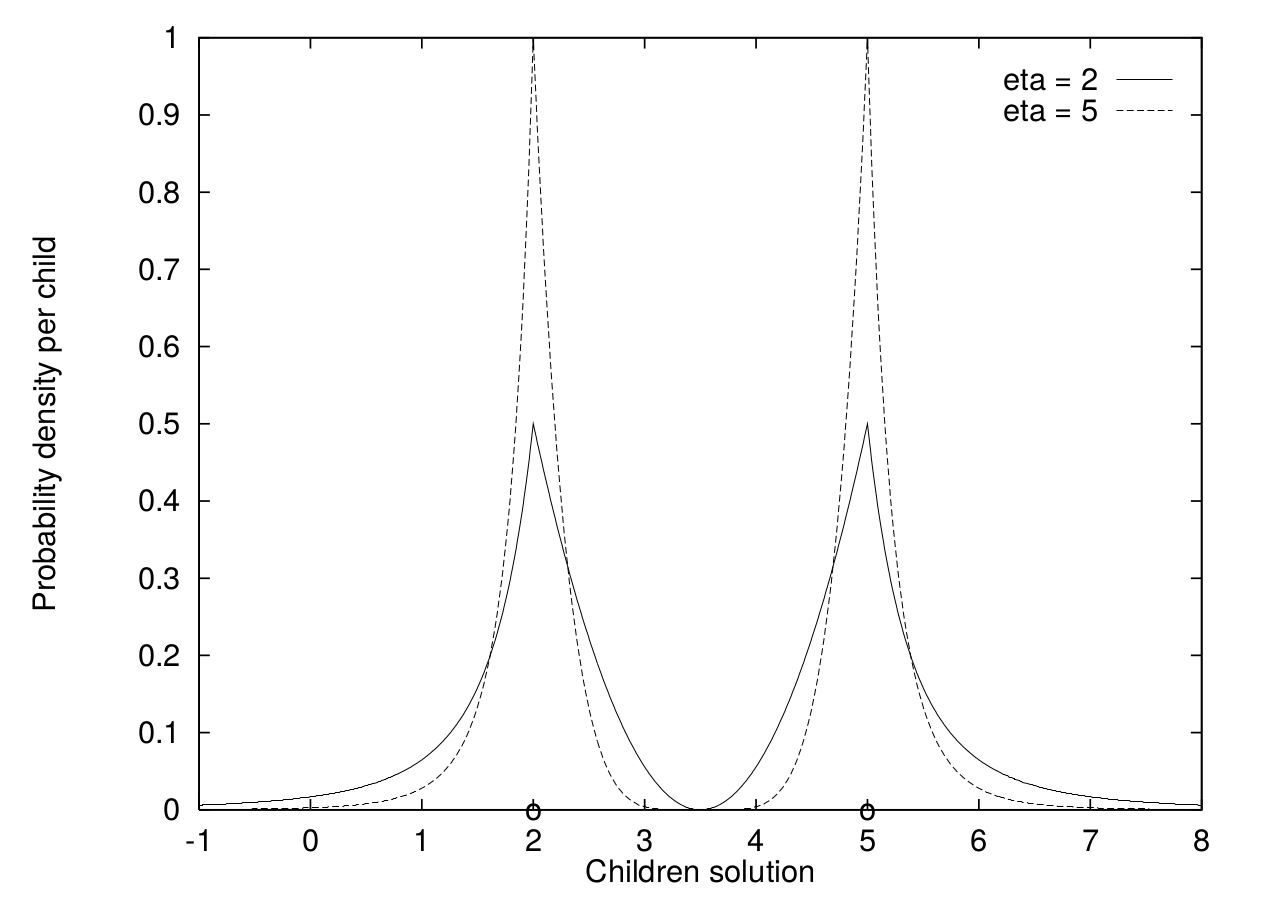
\includegraphics[width=2.5in]{img/DensitySBX_English.png}
\caption{Probability density function SBX with indexes of distribution 2 and 5.}
\label{fig_sim}
\end{figure}


\begin{algorithm}
\algsetup{linenosize=\tiny}
\scriptsize
\caption{Simulated Binary Crossover (SBX)}
\label{alg:SBX_Operator}
\begin{algorithmic}[1]
    \STATE Input: Parents ($P_{1}, P_{2}$), Index distribution ($\eta_c$), Probability distribution ($P_c$).
    \STATE Output: Offsprings ($C_{1}, C_{2}$).
    \IF{ $U[0, 1] \leq P_c$}
       \FOR{ each variable d}
	\IF{ $U[0, 1] \leq  \delta$} \label{alg:inherit_variable}
		\STATE Generate $C_{1,d}$ with equations (\ref{eq:sbx_spread}) and (\ref{eq:child_1}).
		\STATE Generate $C_{2,d}$ with equations (\ref{eq:sbx_spread}) and (\ref{eq:child_2}).
		 \IF{$ U[0, 1]  \geq  \delta $} 
			\STATE Swap $C_{1,d}$ with $C_{2,d}$.
		 \ENDIF
        \ELSE
	   \STATE $C_{1,d} = P_{1, d}$.
	   \STATE $C_{2,d} = P_{2, d}$.
        \ENDIF
       \ENDFOR
    \ELSE
	\STATE $C_{1,d} = P_{1,d}$.
	\STATE $C_{2,d} = P_{2,d}$.
    \ENDIF
\end{algorithmic}
\end{algorithm}


